\section{导数的几何意义}

\begin{theorem}[导数的几何意义]
    导数 $f'(x)$ 的值代表了函数图像在该点切线的斜率。
    \begin{itemize}
        \item 切线越陡峭（正方向），斜率越大；
        \item 越平缓，斜率越接近0；向下倾斜，斜率为负。
    \end{itemize}
\end{theorem}

\begin{example}
    如图，已知函数 $f(x)$ 的图象在点 $P(2,f(2))$ 处的切线为 $l$，则 $f(2) + f'(2) =$ （\quad）
    \begin{center}
        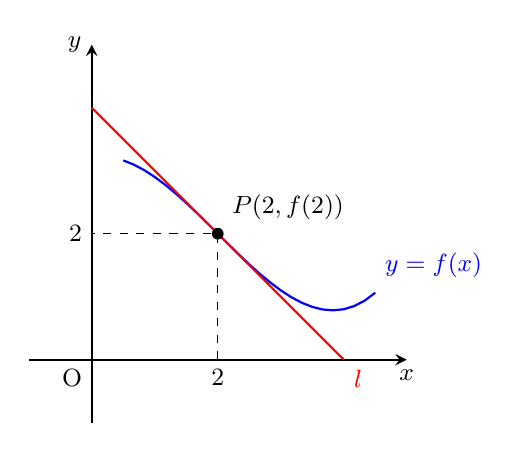
\begin{tikzpicture}[
                scale=0.8,
                >=stealth,
                axis/.style={->, thick},
                font=\small
            ]
            % 坐标轴
            \draw[axis] (-1,0) -- (5,0) node[below] {$x$};
            \draw[axis] (0,-1) -- (0,5) node[left] {$y$};
            \node[below left] at (0,0) {O};

            % --- 调整后的曲线 ---
            % 1. 将常数项从 2.5 改为 2, 确保曲线经过 (2,2)
            % 2. 将三次项系数从 0.25 改为 0.1, 使曲线在切点附近更平缓、更对称
            \draw[blue, thick, domain=0.5:4.5] plot (\x, {0.1*(\x-2)^3 - (\x-2) + 2});
            \node[blue, right] at (4.5, 1.5) {$y=f(x)$};

            % 绘制切线 l，该切线经过 (0,4) 和 (4,0)
            \draw[red, thick] (0,4) -- (4,0) node[below right] {$l$};

            % 标记切点 P (位置不变)
            \node[fill=black, circle, inner sep=1.5pt, label=above right:{$P(2, f(2))$}] at (2,2) {};

            % 辅助虚线 (位置不变)
            \draw[dashed] (2,0) node[below]{2} -- (2,2) -- (0,2) node[left]{2};
        \end{tikzpicture}
    \end{center}
    \begin{tasks}(4)
        \task $- 3$ \task $- 2$ \task 1 \task 2
    \end{tasks}
\end{example}

\v{1em}

\begin{example}
    已知函数 $y = f(x)$ 的图象如图所示，则 $f'(x_{A})$ 与 $f'(x_{B})$ 的大小关系是（\quad）
    \begin{center}
        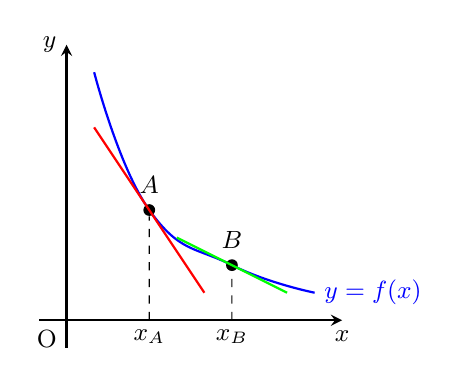
\begin{tikzpicture}[
                scale=0.7,
                >=stealth,
                axis/.style={->, thick},
                font=\small
            ]
            % 坐标轴
            \draw[axis] (-0.5,0) -- (5,0) node[below] {$x$};
            \draw[axis] (0,-0.5) -- (0,5) node[left] {$y$};
            \node[below left] at (0,0) {O};

            % 绘制一个下凹的减函数图像
            \draw[blue, thick] plot[smooth, tension=0.8] coordinates {(0.5,4.5) (1.5,2) (3,1) (4.5,0.5)};
            \node[blue, right] at (4.5,0.5) {$y=f(x)$};

            % 标记点 A 和 B
            \node[fill=black, circle, inner sep=1.5pt, label=above:{$A$}] (A) at (1.5,2) {};
            \node[fill=black, circle, inner sep=1.5pt, label=above:{$B$}] (B) at (3,1) {};
            \draw[dashed] (1.5,0) node[below]{$x_A$} -- (A);
            \draw[dashed] (3,0) node[below]{$x_B$} -- (B);

            % 绘制切线
            \draw[red, thick] (0.5, 3.5) -- (2.5, 0.5);
            \draw[green, thick] (2, 1.5) -- (4, 0.5);
        \end{tikzpicture}
    \end{center}
    \begin{tasks}(2)
        \task $f'(x_{B}) < f'(x_{A}) < 0$
        \task $f'(x_{A}) < f'(x_{B}) < 0$
        \task $f'(x_{A}) = f'(x_{B})$
        \task $f'(x_{A}) > f'(x_{B}) > 0$
    \end{tasks}
\end{example}

\vspace{1em}

\begin{theorem}
    \textbf{导数、割线斜率与函数值的几何关系}:
    \begin{itemize}
        \item $f'(2)$ 和 $f'(3)$ 分别是 $x=2$ 和 $x=3$ 处切线的斜率。
        \item $f(3) - f(2)$ 等于割线斜率 $\frac{f(3)-f(2)}{3-2}$，因为分母为1。
        \item 在此题的凸函数图像上，可以通过比较切线倾斜程度和割线倾斜程度来排序。
    \end{itemize}
\end{theorem}
\begin{example}
    函数 $f(x)$ 的图象如图所示，$f'(x)$ 为函数 $f(x)$ 的导函数，下列数值排序正确的是（\quad）
    \begin{center}
        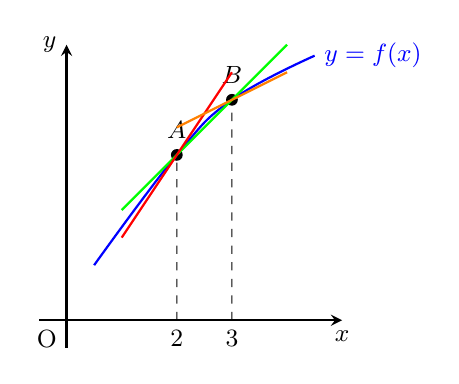
\begin{tikzpicture}[
                scale=0.7,
                >=stealth,
                axis/.style={->, thick},
                font=\small
            ]
            % 坐标轴
            \draw[axis] (-0.5,0) -- (5,0) node[below] {$x$};
            \draw[axis] (0,-0.5) -- (0,5) node[left] {$y$};
            \node[below left] at (0,0) {O};

            % 绘制一个上凸的增函数图像
            \draw[blue, thick] plot[smooth, tension=0.7] coordinates {(0.5,1) (2,3) (3,4) (4.5,4.8)};
            \node[blue, right] at (4.5, 4.8) {$y=f(x)$};

            % 标记点
            \node[fill=black, circle, inner sep=1.5pt, label=above:{$A$}] (P2) at (2,3) {};
            \node[fill=black, circle, inner sep=1.5pt, label=above:{$B$}] (P3) at (3,4) {};
            \draw[dashed] (2,0) node[below]{2} -- (P2);
            \draw[dashed] (3,0) node[below]{3} -- (P3);

            % 绘制割线 AB (代表 f(3)-f(2))
            \draw[green, thick] (1,2) -- (4,5);

            % 绘制 x=2 处的切线
            \draw[red, thick] (1,1.5) -- (3,4.5);

            % 绘制 x=3 处的切线
            \draw[orange, thick] (2,3.5) -- (4,4.5);
        \end{tikzpicture}
    \end{center}
    \begin{tasks}(2)
        \task $0 < f'(2) < f'(3) < f(3) - f(2)$
        \task $0 < f'(3) < f(3) - f(2) < f'(2)$
        \task $0 < f'(3) < f'(2) < f(3) - f(2)$
        \task $0 < f(3) - f(2) < f'(2) < f'(3)$
    \end{tasks}
\end{example}

\vspace{4em}